%%% Hlavní soubor. Zde se definují základní parametry a odkazuje se na ostatní části. %%%

%% Verze pro jednostranný tisk:
% Okraje: levý 40mm, pravý 25mm, horní a dolní 25mm
% (ale pozor, LaTeX si sám přidává 1in)
\documentclass[12pt,a4paper]{report}
\setlength\textwidth{145mm}
\setlength\textheight{247mm}
\setlength\oddsidemargin{15mm}
\setlength\evensidemargin{15mm}
\setlength\topmargin{0mm}
\setlength\headsep{0mm}
\setlength\headheight{0mm}
% \openright zařídí, aby následující text začínal na pravé straně knihy
\let\openright=\clearpage

%% Pokud tiskneme oboustranně:
% \documentclass[12pt,a4paper,twoside,openright]{report}
% \setlength\textwidth{145mm}
% \setlength\textheight{247mm}
% \setlength\oddsidemargin{15mm}
% \setlength\evensidemargin{0mm}
% \setlength\topmargin{0mm}
% \setlength\headsep{0mm}
% \setlength\headheight{0mm}
% \let\openright=\cleardoublepage

%% Pokud používáte csLaTeX (doporučeno):
%\usepackage{czech}
%% Pokud nikoliv:
\usepackage[slovak]{babel} % aby mi nepisalo Obrazek ;-)
%\usepackage[T1]{fontenc}

%% Použité kódování znaků: obvykle latin2, cp1250 nebo utf8:
\usepackage[utf8]{inputenc}

%% Ostatní balíčky
\usepackage{graphicx}
\usepackage{amsthm}
\usepackage{epstopdf}
\newtheorem{theorem}{Veta}
\newtheorem{define}{Definícia}	
\newtheorem{note}{Poznámka}
\newtheorem{example}{Príklad}
\newtheorem{consequence}{Dôsledok}


\usepackage{amsfonts} % matematika
%\usepackage{graphicx} % svg grafika % zbytocne???

\usepackage{graphicx}

% 5 kvoli velkemu Ocku pre casovu zlozitost
\usepackage{amsmath}
\usepackage{amssymb}
\usepackage{mathtools}

\newcommand{\BigO}[1]{\ensuremath{\operatorname{O}\bigl(#1\bigr)}}


% mnoziny
\newcommand{\N}{\mathbb{N}\,}
\newcommand{\Z}{\mathbb{Z}\,}
\newcommand{\Q}{\mathbb{Q}\,}
\newcommand{\R}{\mathbb{R}\,}
\newcommand{\Ri}{\mathbb{R}^{*}\,}


\usepackage{listings} % zdrojaky c++
\usepackage{color}
%\lstset{ %
%language=C++,                % choose the language of the code
%basicstyle=\footnotesize,       % the size of the fonts that are used for the code
%numbers=left,                   % where to put the line-numbers
%numberstyle=\footnotesize,      % the size of the fonts that are used for the line-numbers
%stepnumber=1,                   % the step between two line-numbers. If it is 1 each line will be numbered
%numbersep=5pt,                  % how far the line-numbers are from the code
%backgroundcolor=\color{white},  % choose the background color. You must add \usepackage{color}
%showspaces=false,               % show spaces adding particular underscores
%showstringspaces=false,         % underline spaces within strings
%showtabs=false,                 % show tabs within strings adding particular underscores
%frame=single,           % adds a frame around the code
%framesep=15pt,
%tabsize=2,          % sets default tabsize to 2 spaces
%captionpos=b,           % sets the caption-position to bottom
%breaklines=true,        % sets automatic line breaking
%breakatwhitespace=false,    % sets if automatic breaks should only happen at whitespace
%escapeinside={\%*}{*)}          % if you want to add a comment within your code
%}

\lstset { %
belowcaptionskip=1\baselineskip,
breaklines=true,
language=C++,
showstringspaces=false,
basicstyle=\footnotesize\ttfamily,
keywordstyle=\bfseries\color{green!40!black},
commentstyle=\itshape\color{purple!40!black},
identifierstyle=\color{blue},
stringstyle=\color{orange},
backgroundcolor=\color{black!5}
}


%\usepackage[linesnumbered,ruled,vlined]{algorithm2e}
\usepackage{algorithm}
\usepackage{algorithmic} % http://ftp.cvut.cz/tex-archive/macros/latex/contrib/algorithms/algorithms.pdf
\floatname{algorithm}{Algoritmus}
\renewcommand{\algorithmicrequire}{\textbf{Vstup:}}
\renewcommand{\algorithmicensure}{\textbf{Výstup:}}
\renewcommand{\algorithmiccomment}[1]{\{#1\}}



% \hyphenation{naj-d{\^o}-le-zi-tej-sich}


%% Balíček hyperref, kterým jdou vyrábět klikací odkazy v PDF,
%% ale hlavně ho používáme k uložení metadat do PDF (včetně obsahu).
%% POZOR, nezapomeňte vyplnit jméno práce a autora.
\usepackage[unicode]{hyperref}   % Musí být za všemi ostatními balíčky
\hypersetup{pdftitle=Grid-Based Path Planning}
\hypersetup{pdfauthor=Tomáš Novella}

%%% Drobné úpravy stylu

% Tato makra přesvědčují mírně ošklivým trikem LaTeX, aby hlavičky kapitol
% sázel příčetněji a nevynechával nad nimi spoustu místa. Směle ignorujte.
\makeatletter
\def\@makechapterhead#1{
  {\parindent \z@ \raggedright \normalfont
   \Huge\bfseries \thechapter. #1
   \par\nobreak
   \vskip 20\p@
}}
\def\@makeschapterhead#1{
  {\parindent \z@ \raggedright \normalfont
   \Huge\bfseries #1
   \par\nobreak
   \vskip 20\p@
}}
\makeatother

% Toto makro definuje kapitolu, která není očíslovaná, ale je uvedena v obsahu.
\def\chapwithtoc#1{
\chapter*{#1}
\addcontentsline{toc}{chapter}{#1}
}

\begin{document}

% Trochu volnější nastavení dělení slov, než je default.
\lefthyphenmin=2
\righthyphenmin=2

%%% Titulní strana práce

\pagestyle{empty}
\begin{center}

\large

Univerzita Karlova v Praze

\medskip

Matematicko-fyzikální fakulta

\vfill

{\bf\Large BAKALÁRSKA PRÁCA}

\vfill

\centerline{\mbox{
\includegraphics[width=60mm]{./img/logo.eps}}}

\vfill
\vspace{5mm}

{\LARGE Tomáš Novella}

\vspace{15mm}

% Název práce přesně podle zadání
{\LARGE\bfseries Grid-Based Path Planning}

\vfill

% Název katedry nebo ústavu, kde byla práce oficiálně zadána
% (dle Organizační struktury MFF UK)
Katedra teoretické informatiky a matematické logiky

\vfill

\begin{tabular}{rl}

Vedúci bakalárskej práce: & Mgr. Tomáš Balyo \\
\noalign{\vspace{2mm}}
Študijný program: & Informatika \\
\noalign{\vspace{2mm}}
Študijný obor: & Obecná informatika \\
\end{tabular}

\vfill

% Zde doplňte rok
Praha 2013

\end{center}

\newpage

%%% Následuje vevázaný list -- kopie podepsaného "Zadání bakalářské práce".
%%% Toto zadání NENÍ součástí elektronické verze práce, nescanovat.

%%% Na tomto místě mohou být napsána případná poděkování (vedoucímu práce,
%%% konzultantovi, tomu, kdo zapůjčil software, literaturu apod.)

\openright

\noindent
Poďakovanie.

\newpage

%%% Strana s čestným prohlášením k bakalářské práci

\vglue 0pt plus 1fill

\noindent
Prehlasujem, že som túto prácu vypracoval samostatne a výhradne
s~použitím citovaných prameňov, literatúry a ďalších
odborných zdrojov.


\medskip\noindent
Beriem na~vedomie, že sa na moju prácu vzťahujú práva
a povinnosti vyplývajúce zo zákona  č. 121/2000 Sb.,
autorského zákona a v~platnom znení, obzvlášť skutočnosť,
že Univerzita Karlova v Prahe má právo na~uzavretie licenčnej zmluvy o~použití tejto práce ako školského diela podľa
§60 odst. 1 autorského zákona.

\vspace{10mm}

\hbox{\hbox to 0.5\hsize{%
V ........ dne ............
\hss}\hbox to 0.5\hsize{%
Podpis autora
\hss}}

\vspace{20mm}
\newpage

%%% Povinná informační strana bakalářské práce

\vbox to 0.5\vsize{
\setlength\parindent{0mm}
\setlength\parskip{5mm}

Názov práce:
Grid-Based Path Planning
% přesně dle zadání

Autor:
Tomáš Novella

Katedra:  % Případně Ústav:
Název katedry či ústavu, kde byla práce oficiálně zadána
% dle Organizační struktury MFF UK

Vedúci bakalárskej práce:
Mgr. Tomáš Balyo, Katedra teoretické informatiky a
matematické logiky
% dle Organizační struktury MFF UK, případně plný název pracoviště mimo MFF UK

Abstrakt:
% abstrakt v rozsahu 80-200 slov; nejedná se však o opis zadání bakalářské práce

Kľúčové slová:
% 3 až 5 klíčových slov

\vss}\nobreak\vbox to 0.49\vsize{
\setlength\parindent{0mm}
\setlength\parskip{5mm}

Title:
Grid-Based Path Planning
% přesný překlad názvu práce v angličtině

Author:
Tomáš Novella

Department:
Department of Theoretical Computer Science and Mathematical Logic
% dle Organizační struktury MFF UK v angličtině

Supervisor:
Mgr. Tomáš Balyo, Department of Theoretical Computer Science and
Mathematical Logic
% dle Organizační struktury MFF UK, případně plný název pracoviště
% mimo MFF UK v angličtině

Abstract:
% abstrakt v rozsahu 80-200 slov v angličtině; nejedná se však o překlad
% zadání bakalářské práce

Keywords:
% 3 až 5 klíčových slov v angličtině

\vss}

\newpage

%%% Strana s automaticky generovaným obsahem bakalářské práce. U matematických
%%% prací je přípustné, aby seznam tabulek a zkratek, existují-li, byl umístěn
%%% na začátku práce, místo na jejím konci.

\openright
\pagestyle{plain}
\setcounter{page}{5}
\tableofcontents


%%% Jednotlivé kapitoly práce jsou pro přehlednost uloženy v samostatných souborech
\chapter*{Úvod}
\addcontentsline{toc}{chapter}{Úvod}

Slávna Eulerova úloha siedmych kaliningradských mostov sa považuje za prvú prácu, 
ktorá zaviedla teóriu grafov. Úlohou je prejsť to týchto siedmych mostoch tak, aby sme po každom šlo práve raz.
Od tej doby sa využitie teórie grafov značne
rozšírilo a v dnešnej dobe patrí medzi významné
a rozpracované teórie. V modernej dobe jedným z jej 
najdôležitejších problémov je hľadanie najkratšej cesty. Najčastejšie sa s nimi stretávame pri 
GPS navigacii.
Medzi najvýznamnešie práce považujeme práce od Dijkstru a Floyd-Warshalla.

S narastajúcim fenoménom počítačových hier 
a umelej inteligencie sa do povedomia dostal špeciálny typ grafu --
mriežkový graf, využívaný ako herná mapa.
V hrách trebalo často nájsť cestu pre počítačom
ovládanú postavičku z miesta A do miesta B.
Nakoľko je ale väčšina hier komerčná, algoritmy
využívané v hrách boli a sú taktiež komerčne.
Dôsledkom toho nie sú publikované a porovnané rôzne prístupy a algoritmy
na vyhľadávanie v mriežkových mapách. A keď už aj sú, tak práce používajú rôzne mapy
na bechmarking a teda neexistuje žiadna globálna porovnávacia štúdia týchto prístupov.
Tento problém sa snažil vyriešiť GPPC - Grid-Based Path Planning Competition - teda súťaž, ktorá porovnáva rôzne algoritmy na veľkej množine máp
použitých v známych počítačových hrách.

Cieľom tejto práce je spraviť prehľad doterajších prístupov k tomuto problému a prispieť vlastným algoritmom
do súťaže.




V práci sme naimplementovali vlastný algoritmus a porovnali ho s doterajšímy známymi.
TODO?? Počas práce sme prišli na zaujímavé zefektívnenie algoritmov [snad na nieco prijdem :))]a dúfame v jeho rozšírenie do hernej sféry.

ASK?? ake su vlastne ciele? mam vymysliet vzbrusu novy algoritmus?

V prvej kapitole si zadefinujeme kľúčové termíny a popíšeme problem. Na konci kapitoly spomenieme súťaž, ktorej sa daný algoritmus zúčastnil 
a popíšeme jej podmienky.
Druhá kapitola sa pokúsime rozobrať doterajšie zistenia a algoritmy používané na riešenie obdobných problémov.
V tretej kapitole popíšeme náš algoritmus a vo štvrtej kapitole ho porovnáme s ostatnými algoritmami a uvedieme výsledky.

\chapter{Zadanie problému a cieľové požiadavky}

\section{Úvodné definície a značenia}
Na začiatok si zaveďme niektoré dôležité pojmy z teórie grafov.
Budú sa týkať obecnej teórie a úlohu so všetkými jej špecifikami si ozrejmíme v nasledujúcej kapitole.
\begin{define}
{\sl Graf G} je usporiadaná dvojica (V, E), kde V označuje množinu vrcholov(vertices) a $E \subseteq V \times V $ označuje množinu hrán (edges). Značíme G = (V, E).
\end{define}

\begin{define}
{\sl Ohodnotený graf (G, w)} je graf s spolu s reálnou funkciou (tzv. ohodnotením)
$w: E(G) \to \R$, kde $w$ je funkcia, ktorá každej hrane priradí
reálne číslo, takzvanú \emph{cenu}, alebo \emph{dĺžku} hrany.
\end{define}
ukazka na \ref{fig:ohodnoteny_graf}

\begin{figure}[h]
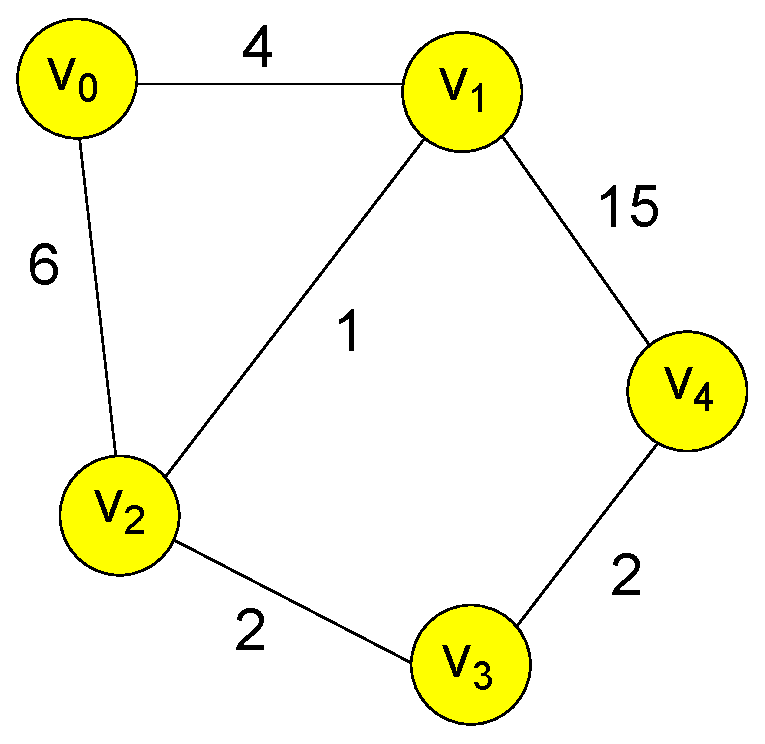
\includegraphics[height=7.5cm]{./img/graf.eps}
\caption{Ohodnotený graf}
\label{fig:ohodnoteny_graf}
\end{figure}

Teraz keď už vieme, čo je to graf, skúsme si zadefinovať najkratšiu cestu. Začnime najprv obecne cestou.

\begin{define}
{\sl Cesta P z vrcholu $v_0$ do vrcholu $v_n$ v grafe G } je postupnosť $P = (v_{0},e_{1},v_{1},\dots, e_{n}, v_{n})$,
pre ktorú platí $e_{i} = \{v_{i-i},v_{i}\}$ a taktiež
$v_{i} \ne v_{j}$ pre každé $i \ne j$.
\end{define}






Všimnime si, že v ceste nenavštívime žiaden vrchol dvakrát a teda cesta neobsahuje kružnice.

TODO?? dlzka hrany - cena cesty - zadefinuj funkciu d(u, v)

\begin{define}
{\sl Cena cesty P z vrcholu $v_0$ do vrcholu $v_n$ v ohodnotenom grafe (G, w) } je súčet cien hrán, ktoré sa na ceste nachádzajú.
\end{define}

\begin{define}
{\sl Najkratšia cesta P z vrcholu $v_0$ do vrcholu $v_n$
v ohodnotenom grafe (G, w)} 
je cesta s najnižsou cenou.
\end{define}





\section{Mriežkový graf}

Po zavedení kľúčových pojmov sa dostávame k samotnému zadaniu úlohy. 
Ako sme už spomínali, problém budeme riešit na tzv. mriežkových grafoch. Čo je mriežkový graf a v čom sa od obecného grafu odlišuje?

Zjednodušene povedané, je to mapa s ktorou sa stretávame v najrôznejších hrách, ako je Warcraft, Startcraft, Dragon Age
a~podobne. ASK?? je to "mapa" dat do uvodzoviek

Ide o špeciálny a dosť obmedzený typ grafu. Vizuálne si ho môžme predstaviť ako konečný graf v ktorom sú vrcholy rozostúpené v tvare mriežky a hrana
je stále medzi dvojicami susedných vrcholov vo všetkých ôsmych smeroch. Cena vodorovnej alebo zvislej hrany je $1$ a cena šikmej hrany je $\sqrt{2}$.


\begin{figure}[h]
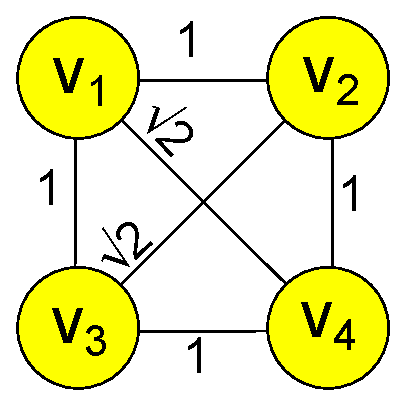
\includegraphics[height=5.5cm]{./img/herna_mapa2x2.eps}
\caption{Mriežkový graf 2x2}
\label{fig:mriezkovy_graf2x2}
\end{figure}


\begin{figure}[h]
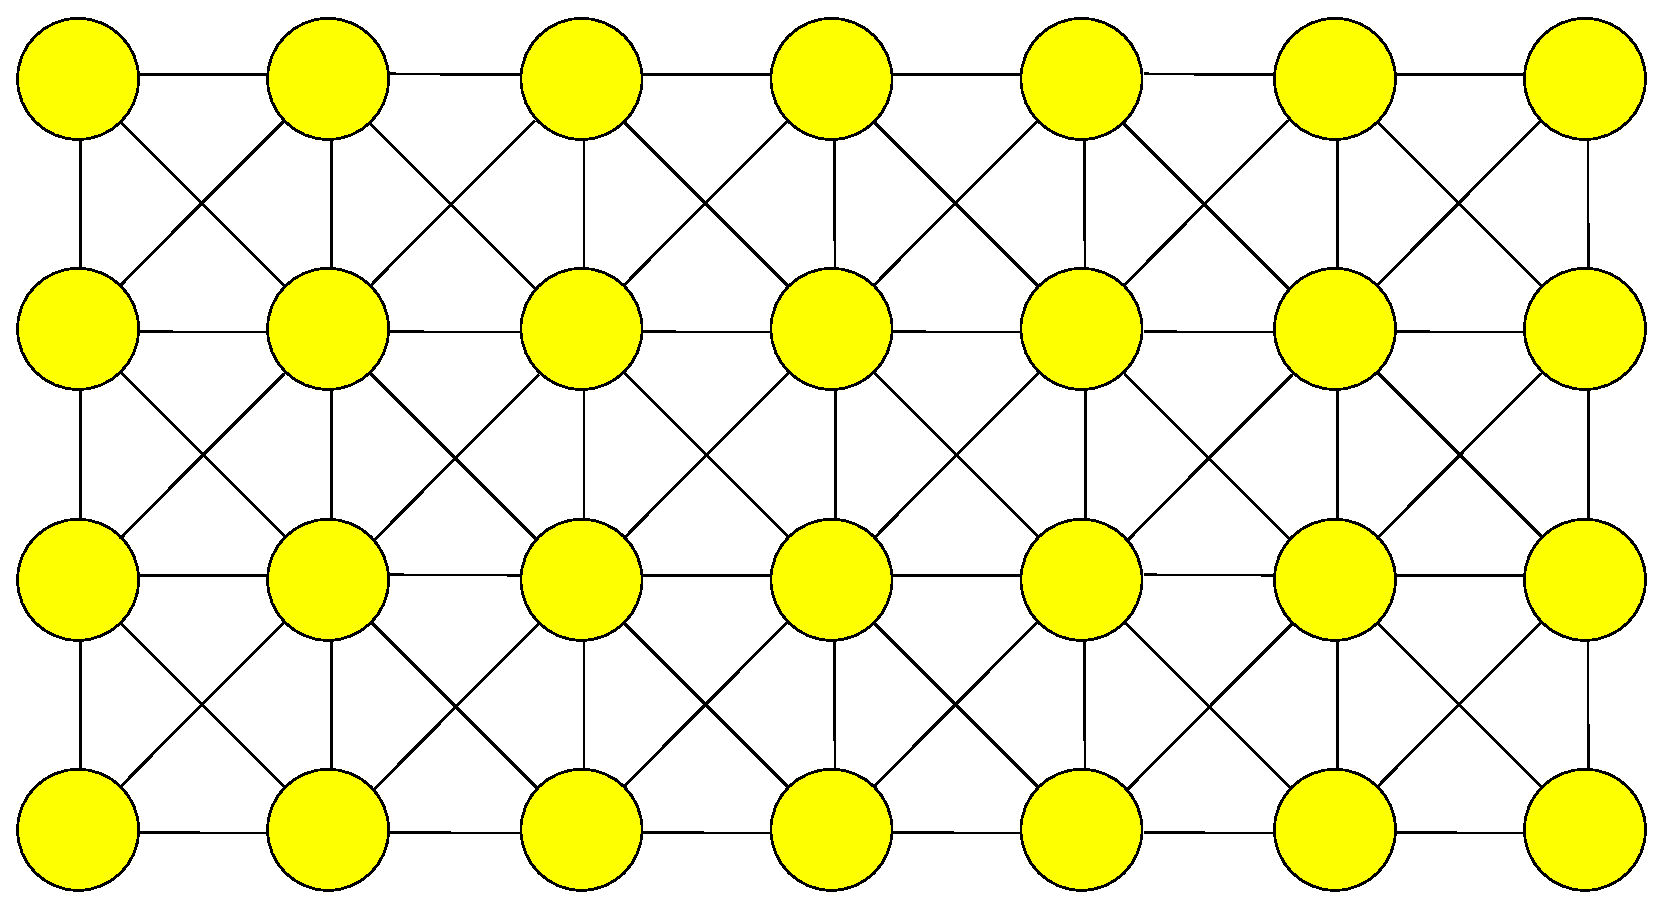
\includegraphics[height=5.5cm]{./img/herna_mapa.eps}
\caption{Mriežkový graf bez označenia vrcholov a dĺžok hrán}
\label{fig:mriezkovy_graf}
\end{figure}


Zadefinujme si teraz mriežkový graf formálne.

\begin{define}
{\sl Mriežkový graf rozmerov m*n} je ohodnotený graf v ohodnotením $w$ s m*n vrcholmi očíslovanými od $v_{1,1}$ až po $v_{m,n}$ 
s~jednoduchými hranami $j$ v~tvare $\{v_{a,b}, v_{a,b+1}\}, \{v_{a,b}, v_{a+1,b}\}$, kde $w(j) = 1$ 
a šikmými hranami $ s $ v~tvare 
$\{v_{a,b}, v_{a+1,b+1}\}$, $\{v_{a,b}, v_{a+1,b+1}\}$, kde $ w(s) = \sqrt{2}$.
\end{define}

FIXME?? pridat obrazky

\begin{note}
	Mriežkový graf sa dá reprezentovať ako matica m*n nad telesom $\Z_2$, kde jednotky predstavujú vrcholy. Príklad maticovej reprezentácie grafu rozmerov 4x5 je na obrázku
	\ref{fig:maticova_reprezentacia}.
\end{note}



\begin{figure}[h]
\caption{Maticová reprezentácia mriežkového grafu}
\label{fig:maticova_reprezentacia}
\[
G =
  \begin{bmatrix}
    0 & 0 & 1 & 1 & 1 & 1\\
	0 & 0 & 1 & 1 & 1 & 0\\
	0 & 0 & 0 & 1 & 1 & 1\\
	0 & 0 & 0 & 0 & 0 & 0\\
  \end{bmatrix}
\]
\end{figure}




\section{GPPC: Grid-Based Path Planning Competition}
Algoritmus navrhnutý a naprogramovaný v tejto práci bol zaradený do súťaže \textbf{GPPC}, ktorá sa koná približne 2 krát ročne.

\subsection{Špecifiká súťaže, limity}

Herné mapy budú mať rozmery maximálne $2048 \times 2048$.
Súťaž bude rozdelená do dvoch fáz --- fázy predspracovania mapy(pre-processing)
a fázy testovania. Na predspracovanie mapy bude vyhradený čas
maximálne 30 minút a program si svoje dáta uloží na disk do súboru o veľkosti maximálne 50MB.
A potom vo fáze testovania budé dostávať požiadavky na nájdenie najkratšej cesty.

Úlohou súťaže je naimplementovať tieto tri funkcie.

\lstset{language=C++}          % Set your language (you can change the language for each code-block optionally)

\begin{lstlisting} %[frame=single]  % Start your code-block

void PreprocessMap(std::vector &bits, int width, int height,
                   const char *filename);
                   
void *PrepareForSearch(std::vector &bits, int width, int height,
                       const char *filename);
bool GetPath(void *data, xyLoc s, xyLoc g, std::vector &path);
\end{lstlisting}

\subsection{Kritériá súťaže, hodnotenie programov}
Programy sa nebudú porovnávať v jednej metrike a podľa jedného
kritéria, nakoľko sa programy dalo zoptimalizovať podľa viacerých kritérií. Metriky sú nasledovné:

\begin{itemize}
\item Celkový čas na~nájdenie cesty.
\item Čas na nájdenie prvých 20 tich krokov.
\item Dĺžka cesty (zohľadnená suboptimalita).
\item Maximálny čas vrátenia hociktorej časti cesty.
\end{itemize}

Testovací počítač má 12 GB RAM pamäti a dva 2.4 Ghz Intel Xeon E5620
procesory.
\chapter{Prehľad algoritmov}
Na hľadanie najkratších ciest v grafe poznáme mnoho algoritmov, ktoré vieme rozdeliť do troch skupín.


\begin{itemize}
\item Point To Point Shortest Path - hľadajú najkratšiu cestu medzi dvoma zadanými bodmi
\item Single Source Shortest Path - pre daný vrchol {\sl v} hľadajú najkratšiu cestu do všetkých vrcholov grafu.
\item All Pairs Shortest Path - skúmajú najkratšiu cestu medzi všetkými dvojicami vrcholov.
\end{itemize}

Napriek tomu, že sú tieto problémy na obecných grafoch NP-ťažké, na mriežkových grafoch, kde majú všetky vrcholy kladnú cenu, vieme nájsť riešenie v polynomiálnom čase.
V práci sa budeme ďalej zaoberať riešením prvého problému (Point to Point Shortest Path).

V tejto kapitole si popíšeme algoritmy, ktoré sú použiteľné na všetkých grafoch 
s nezápornými dĺžkami hrán.

\section{Dijkstrov algoritmus}
Medzi základné algoritmy patrí Dijkstrov algoritmus, ktorý je asymptoticky optimálny (TODO?? for sure?).

Pri hľadaní cesty z vrcholu $s$ do vrcholu $t$ prechádzame postupne vrcholy zo stúpajúcou vzdialenosťou od $s$, až dokým sa nedostaneme k cieľovému vrcholu $t$.
Vizuálne si beh algoritmu môžme predstaviť ako kruh so stredom v bode $s$ so zväčšujúcim sa polomerom. Algoritmus napísaný v pseudokóde je nasledovný:


\begin{algorithm}
\caption{Dijkstra: Nájdi najkratšiu cestu medzi dvoma bodmi {\sl s} a {\sl t}}
\label{alg:dijkstra}
\begin{algorithmic}[1] % number one = line numbering is on
\REQUIRE $s=(x_s,y_s), t=(x_t,y_t)$
\ENSURE $path$


\STATE path.append($(x_s, y_s)$)
\COMMENT {pridám počiatok}

\WHILE {$x_s \neq x_t \vee y_s \neq y_t $}
	\IF {$x_s \textless x_t$}
		\STATE $x_s \leftarrow x_s + 1$
	\ELSIF {$x_s \textgreater x_t$}
		\STATE $x_s \leftarrow x_s - 1$
	\ENDIF

	\IF {$y_s \textless y_t$}
		\STATE $y_s \leftarrow y_s + 1$
	\ELSIF {$y_s \textgreater y_t$}
		\STATE $y_s \leftarrow y_s - 1$
	\ENDIF
	\STATE path.append($(x_s, y_s)$)
\ENDWHILE

\end{algorithmic}
\end{algorithm}



\section{Lineárny Dijkstrov algoritmus}
Môž


\section{A*}
dalsi algoritmus do zbierky je a* \cite{astar72}.

\chapter{Nový algoritmus: NovellA*}

\section{Zlepšenie výkonu v niektorých prípadoch}
Nie všetky cesty sú ale také kľukaté. V mnohých prípadoch, napríklad keď medzi počiatočným a koncovým bodom neleží žiadna prekážka, 
sú cesty veľmi priamočiare. To sa pokúsime využiť na zlepšenie výkonu algoritmu v~niektorých prípadoch. 
Predstavme si, že máme obdlžníkovú mapu bez prekážoch a hľadáme najkratšiu cestu medzi bodmi $s=(x_s,y_s), t=(x_t,y_t)$.
V tomto prípade vieme nájsť najkratšiu cestu veľmi jednoducho.
Algoritmus:
vstup: \\
$s=(x_s,y_s), t=(x_t,y_t)$ \\
vystup:\\
path \dots usporiadaná množina súradníc po ktorých vedie cesta\\
beh algoritmu:\\


\lstset{language=Python}          
\begin{lstlisting} %[frame=single]  

path = (xs, ys)

# skopirujem súradnice zdrojového vrcholu
(x1, y2) = (xs, ys) 
while (x1, y1) <> (x2, y2):
	if y1 < y2:
		++y1
	else:
		--y1

	if x1 < x2:
		++x1
	else:
		--x1
	path.append((x1,y1))
\end{lstlisting}

Teda, jednoducho povedané: keď sa počiatočný a koncový bod líšia v jednej súradnici, tak sa posúvame priamočiaro,
keď sa líšia v oboch, tak sa posúvame šikmo.

Pokiaľ si zadefinujeme $dx := \abs{x_t - x_s}$ a $dy := \abs{y_t - y_s}$, tak počet vrcholov,
ktorými cesta prechádza vieme zhora odhadnúť, ako $\max(dx, dy)$. Jej vzdialenosť vieme zistiť v čase  $\BigO{\max(dx, dy)}$
Na zistenie vzdialenosti v každom kroku nám stači konštantná pamäť.

TODO?? Poznamka, ze nepotrebujem na to obdlzniky, mozem robit aj komplikovanejsie utvary, ale by to sa blbo hladalo... ledaze...

Skúsme to teda nejak využiť. Pokiaľ vieme, že počiatočný aj koncový bod ležia v jednom obdĺžniku, tak máme problém vyriešený. 
Jediným problémom ostalo takéto obdĺžniky nájsť. 


ASK?? alebo radsej neutralne napiast, hladanie obdlznikov?
\section{Hľadáme obdĺžniky}

Pre ľahšie vyjadrovanie si zaveďme definíciu {\sl čistej hernej mapy}.

\begin{define}
{\sl Herná podmapa je čistá} 
pokiaľ medzi každými dvoma susednými vrcholmi existuje hrana.
\end{define}

Naformulujme si teda problém exaktne. Chceme na vstupnej mape nájsť obdĺžniky, aby spolu mali čo najväčší obsah a aby ich bolo čo najmenej.
ASK?? teda staci mi spravit obdlzniky 1x1 a potmo ich spajat...to je ako vsetko?
\chapter{Porovnanie algoritmu NovellA* s ostatnými algoritmami.}

\section{Vstupné dáta}
Častým problémom pri vzájomnom porovnávaní algoritmov je
nájsť tetsovaciu vyorku, ktor... \cite{sturtevant2012benchmarks}


Na porovnávanie využijeme benchmark

TODO?? bibliografia styl - priezvisko,meno - alebo naopak???
\chapter{T-maps - Vizuálna predstava}

Pre názornejšiu predstavu behu algoritmu sme navrhli softvér \textbf{T-maps}, ktorý beh algoritmov ilustruje graficky.

\section{Použitie}

Program T-maps  Na začiatku do neho nahrajeme mapu, nad ktorou algoritmus beží a taktiež dáta
tohto algoritmu (prehľadané vrcholy a najkratšiu cestu) a program tieto hodnoty graficky znázorní.
Medzi možnosti programu patrí export mapy a viditeľného poľa do súboru.
 TODO??  uzivatelska dokumentacia
Mozno popis zaujimavej casti  


% Ukázka použití některých konstrukcí LateXu (odkomentujte, chcete-li)
%%% Ukázka použití některých konstrukcí LaTeXu

\subsection{Ukázka \LaTeX{}u}
\label{ssec:ukazka}

V~této krátké části ukážeme použití několika základních konstrukcí \LaTeX{}u,
které by se vám mohly při psaní práce hodit.

Třeba odrážky:

\begin{itemize}
\item Logo Matfyzu vidíme na obrázku.~\ref{fig:mff}
\item Tato subsekce má číslo~\ref{ssec:ukazka}.
\item Odkaz na literaturu~\cite{lamport94}.
\end{itemize}

Druhy pomlček:
červeno-černý (krátká),
strana 16--22 (střední),
$45-44$ (minus),
a~toto je --- jak se asi dalo čekat --- vložená věta ohraničená dlouhými pomlčkami.
(Všimněte si, že jsme za \verb|a| napsali vlnovku místo mezery: to aby se
tam nemohl rozdělit řádek.)

% Makro na české uvozovky (novější verze LaTeXu ho už mají zabudované)
%\newcommand{\uv}[1]{\quotedblbase #1\textquotedblleft}
\uv{České uvozovky.}

%\newtheorem{theorem}{Věta}
%\newtheorem*{define}{Definice}	% Definice nečíslujeme, proto "*"

\begin{define}
{\sl Strom} je souvislý graf bez kružnic.
\end{define}


\begin{theorem}
Tato věta neplatí.
\end{theorem}


\begin{proof}
Neplatné věty nemají důkaz.
\end{proof}

\begin{figure}
	\centering
	
\includegraphics[width=30mm]{./img/logo.eps}
	\caption{Logo MFF UK}
	\label{fig:mff}
\end{figure}



\chapter*{Záver}
\addcontentsline{toc}{chapter}{Záver}


%%% Seznam použité literatury
%%% Seznam použité literatury je zpracován podle platných standardů. Povinnou citační
%%% normou pro bakalářskou práci je ISO 690. Jména časopisů lze uvádět zkráceně, ale jen
%%% v kodifikované podobě. Všechny použité zdroje a prameny musí být řádně citovány.

\def\bibname{Zoznam použitej literatúry}
\begin{thebibliography}{99}
\addcontentsline{toc}{chapter}{\bibname}
%%%%

\bibitem{euler41}
	L. Euler. 
	\emph{Solutio problematis ad geometriam situs pertinentis}.
    Commentarii academiae scientiarum Petropolitanae, 8:128–140, 1741.

\bibitem{dijkstra59}
  E. W. Dijkstra.
  \emph{A note on two problems in connexion with graphs}.
  Numerische Mathematik, 1(1):269--271, 1959.

\bibitem{floyd62}
Robert~W. Floyd.
\newblock Algorithm 97: Shortest path.
\newblock {\em Commun. ACM}, 5(6):345--, June 1962.



\bibitem{mares07}
  M. Mareš.
  \emph{Nejkratší cesty}.
  Krajinou grafových algoritmů, 2007.
  
\bibitem{astar72}
Peter~E. Hart, Nils~J. Nilsson, and Bertram Raphael.
\newblock Correction to a formal basis for the heuristic determination of minimum cost paths.
\newblock {\em SIGART Bull.}, (37):28--29, December 1972.

\bibitem{golberg01}
A. V. Goldberg. 
\emph{Shortest Path Algorithms: Engineering Aspects}. 
In Proc. ESAAC '01, Lecture Notes in
Computer Science. Springer-Verlag, 2001.


\bibitem{goldbergharrelson05}
A. V. Goldberg and C. Harrelson. 
\emph{Computing the Shortest Path: A* Search Meets Graph Theory}.
In Proc. 16th ACM-SIAM Symposium on Discrete Algorithms, pages 156--165, 2005.

\bibitem{asymptotic65}
 J. Hartmanis, R. Stearns. 
 \emph{On the computational complexity of algorithms}. 
 Transactions of the American Mathematical Society, vol. 117, 285--306, 1965.

\bibitem{sturtevantgppc}
  N.~Sturtevant.
  \emph{GPPC: Grid-Based Path Planning Competition}.
  Dostupné z: \url{http://http://movingai.com/GPPC/} 
   
\bibitem{sturtevant2012benchmarks}
N.~Sturtevant.
\newblock Benchmarks for grid-based pathfinding.
\newblock {\em Transactions on Computational Intelligence and AI in Games},
  4(2):144 -- 148, 2012.
   
\bibitem{gs97}
A.~Goldberg, C. Silverstein.
\emph{Implementations of Dijkstra’s Algorithm Based on Multi-Level Buckets}.
Springer Berlin Heidelberg,
1997.
\end{thebibliography}


%%% Tabulky v bakalářské práci, existují-li.
\chapwithtoc{Zoznam tabuliek}

%%% Použité zkratky v bakalářské práci, existují-li, včetně jejich vysvětlení.
\chapwithtoc{Zoznam použitých skratiek}

%%% Přílohy k bakalářské práci, existují-li (různé dodatky jako výpisy programů,
%%% diagramy apod.). Každá příloha musí být alespoň jednou odkazována z vlastního
%%% textu práce. Přílohy se číslují.
\chapwithtoc{Prílohy}

\openright
\end{document}
